\documentclass{beamer}
\usepackage[utf8]{inputenc}
\usepackage{xeCJK} 
\usepackage[T1]{fontenc}
\usepackage{mathabx}
\usepackage{amsmath} 
\usepackage{mathpazo}
\usepackage{bibentry}
\usepackage{tikz}
\usepackage{caption}
\usepackage{graphicx}
\usepackage{subfigure}
\usepackage{animate}
\usepackage{hyperref}

\usetikzlibrary{scopes}
\def\iangle{35} % Angle of the inclined plane
\def\down{-90}
\def\arcr{0.5cm} % Radius of the arc used to indicate angles

\usetheme{Boadilla}
\usecolortheme{wolverine}
\useoutertheme{miniframes}

\title{VP160 Recitation Class VII}
\subtitle{Angular Momentum \& Rigid Body Dynamics Part I}
\author{Zeyi Ren}
\institute{UM-SJTU Joint Institute}

\begin{document}

\maketitle

\frame{\tableofcontents}

\section{Angular Momentum}
\begin{frame}
  \begin{block}{Angular Momentum}
    $$\vec{L} = \vec{r}\times \vec{p}$$
    $$[kg\cdot m^2/s]$$
  \end{block}
  \pause
How to derive?
$$\vec{F} = \frac{d\vec{p}}{dt}$$\pause
$$\Rightarrow \vec{r}\times \vec{F} = \vec{r}\times \frac{d\vec{p}}{dt} = \frac{d}{dt}(\vec{r}\times \vec{p}) - \frac{d\vec{r}}{dt}\times \vec{p}$$\pause
$$
\text{Notice }\frac{d\vec{r}}{dt}\times \vec{p}=\vec{v}\times (m\vec{v}) = 0 
$$\pause
$$\Rightarrow \underbrace{\vec{r}\times \vec{F}}_{\vec{\tau}} = \frac{d}{dt}\underbrace{\vec{r}\times \vec{p}}_{\vec{L}}$$
$$\vec{\tau}\text{: torque}$$
$$[N\cdot m]$$
\end{frame}

\begin{frame}
  \begin{block}{Angular Momentum Theorem}
    $$\vec{\tau} = \frac{d\vec{L}}{dt}\Rightarrow \vec{L}(t_2) - \vec{L}(t_1) = \int_{t_1}^{t_2}\vec{\tau}dt$$
  \end{block}\pause
  \begin{block}{Law of Conservation of Angular Momentum}
    $$\text{If }\vec{\tau} = 0\Rightarrow \vec{L} = \text{const}$$
  \end{block}\pause
  Applications: 
  \begin{itemize}
    \item Central force field ($\vec{\tau} = \vec{r}\times \vec{F} = 0$)\pause
    \item Aerial velocity, e.g. motion of planets, Kepler's Second Laws 
  \end{itemize}
\end{frame}

\begin{frame}
  \begin{figure}[htbp]
  \centering
  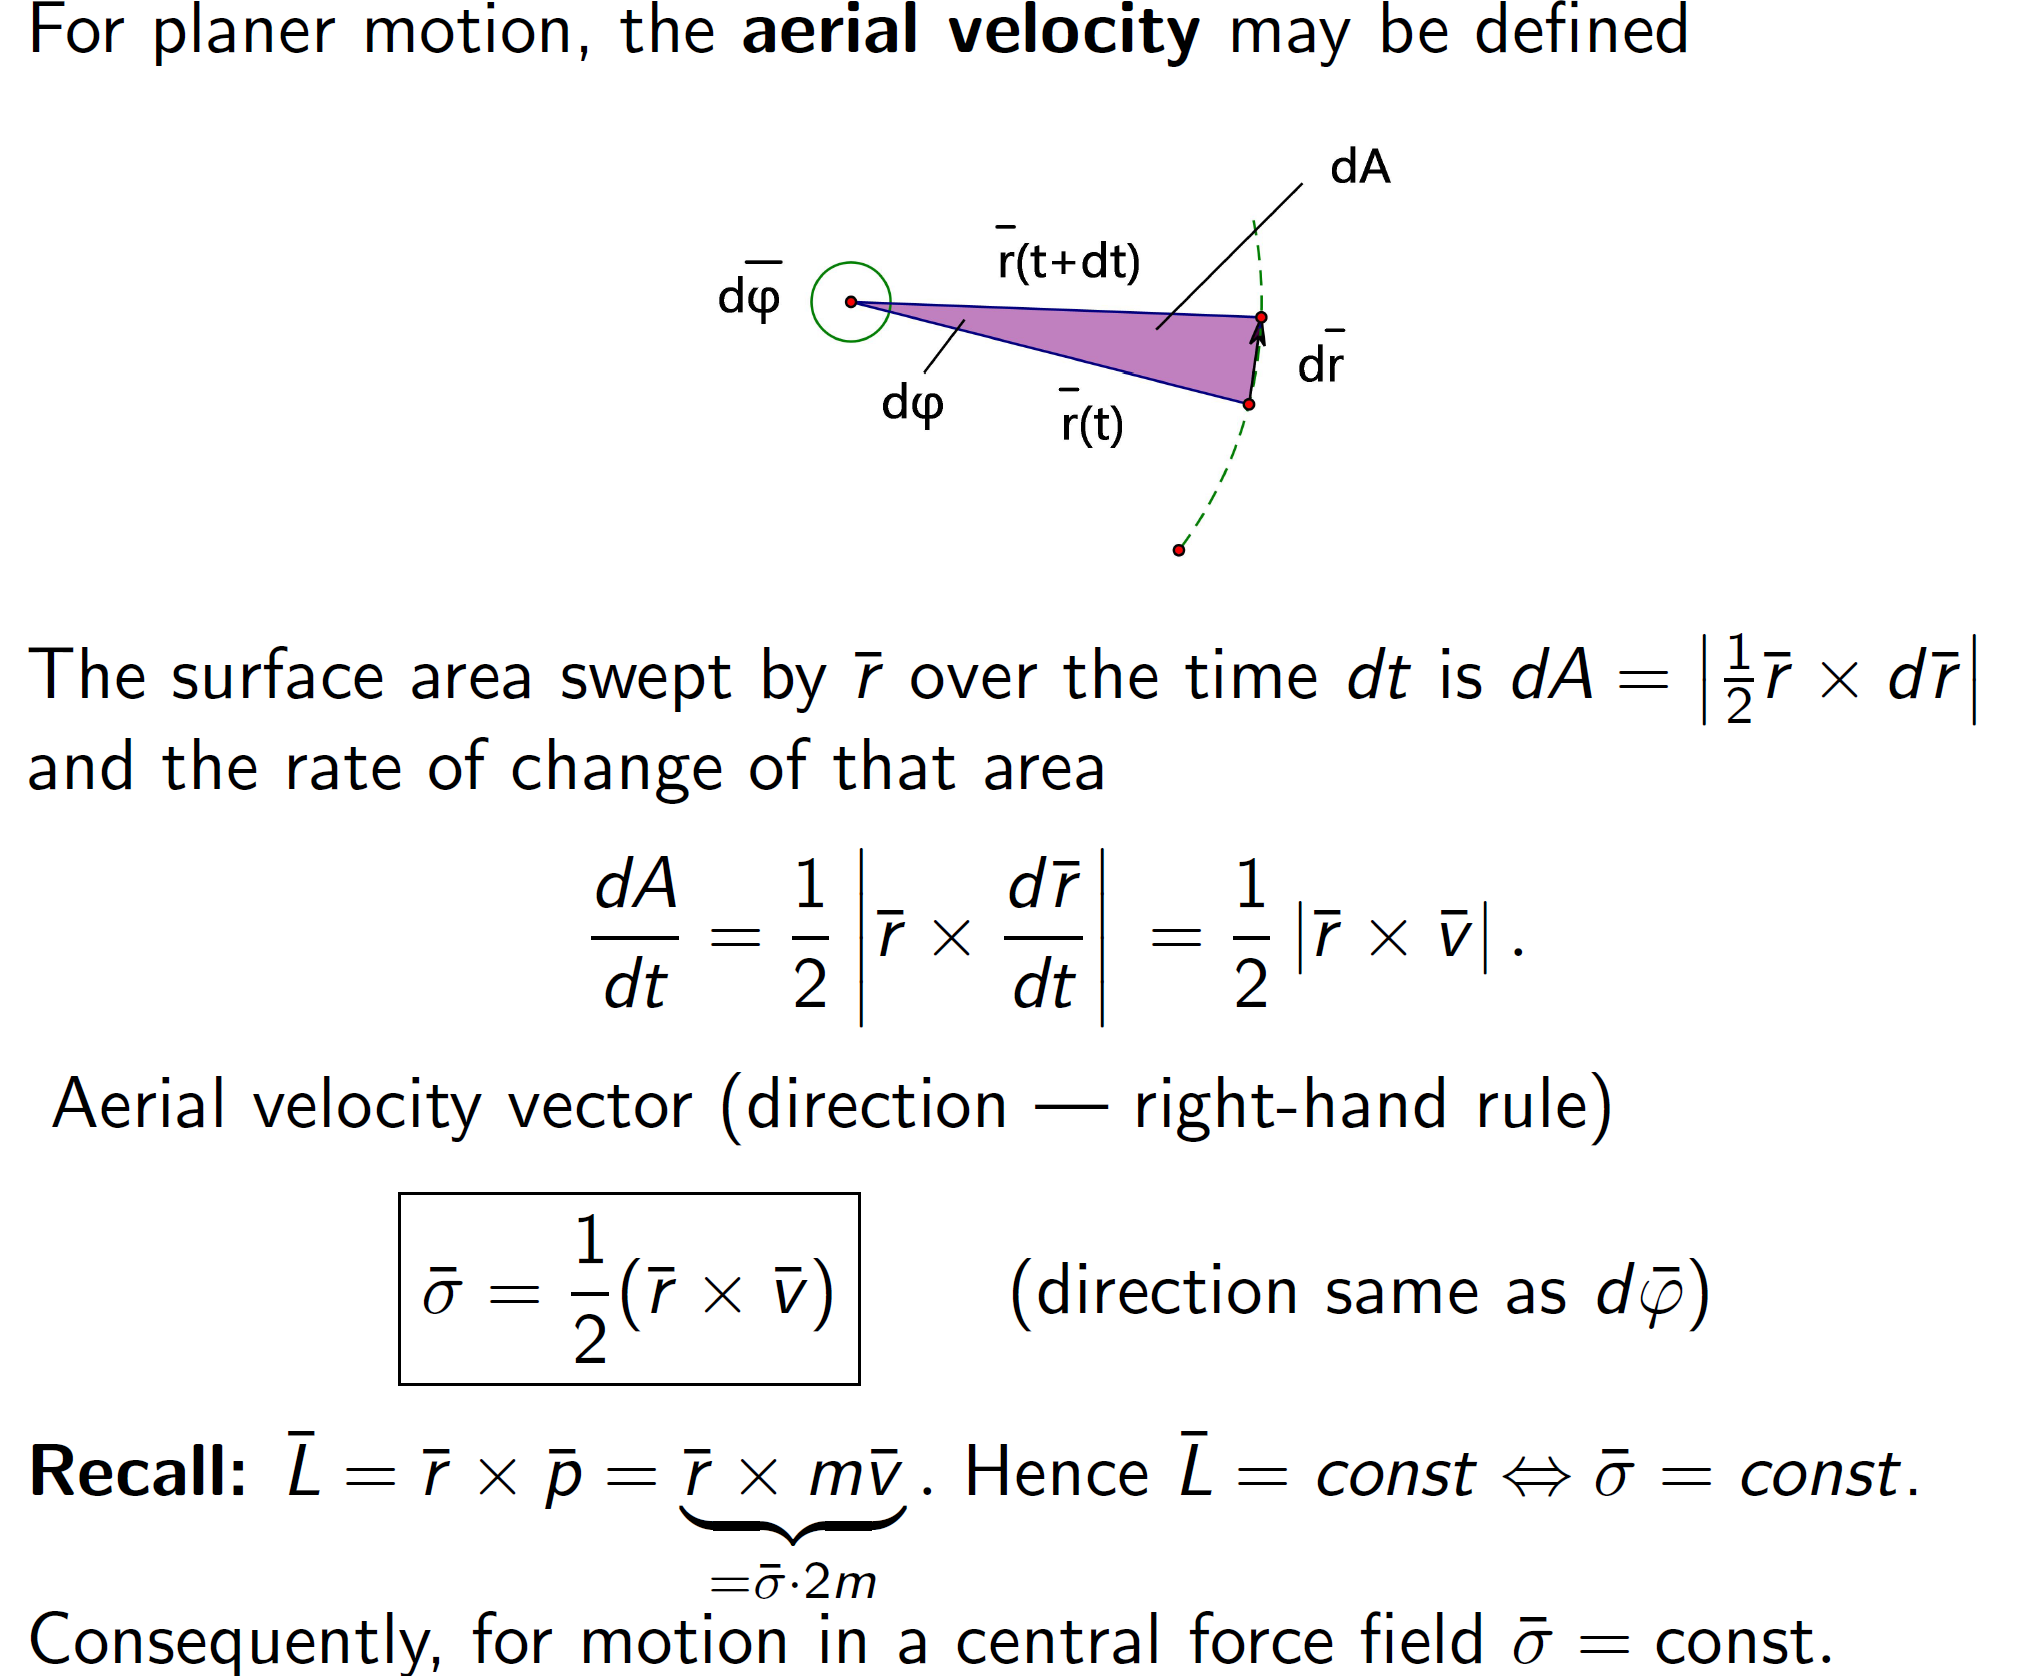
\includegraphics[width=0.78 \linewidth, angle =0]{Aerial.png}
  %\caption{.}
  \label{fig:1}
  \end{figure}
\end{frame}

\begin{frame}{Angular Momentum in System of Particles}
  \begin{block}{Conservation of the Angular Momentum Law}
    If the net torque of external forces on a system of particles is equal to zero, then the total angular momentum of that system is conserved.
  \end{block}\pause
  $$\frac{d\vec{L}}{dt} = \vec{\tau} = \vec{\tau_{ext}} + \underbrace{\vec{\tau_{int}}}_{= 0}$$\pause
  \textcolor{blue}{Why $ \vec{\tau_{int}}= 0$?} \\
  For any two particles $k, l$ in the system,
  $$\vec{\tau_{k\rightarrow l}} = -\vec{\tau_{l\rightarrow k}}$$
  \begin{figure}[htbp]
  \centering
  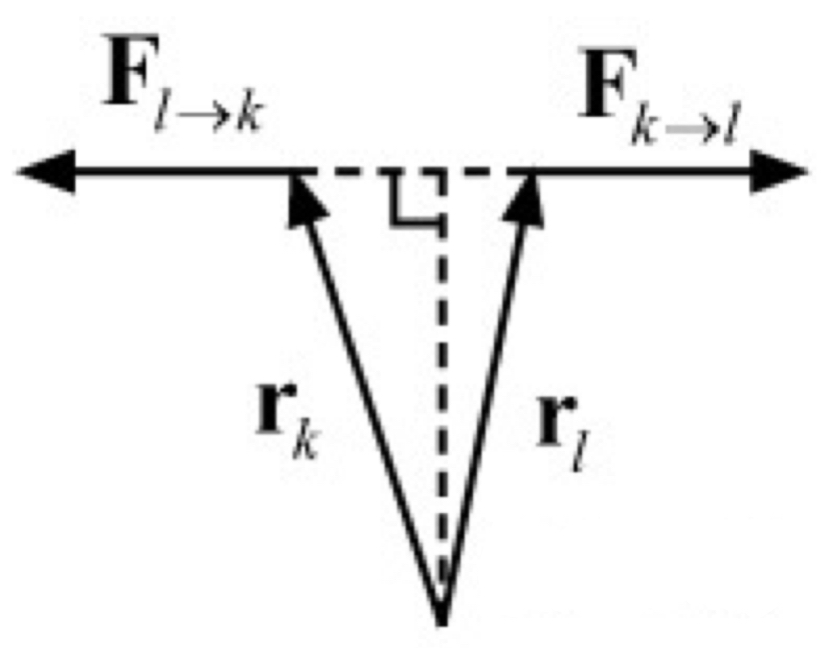
\includegraphics[width=0.15 \linewidth, angle =0]{prove.png}
  %\caption{.}
  \label{fig:2}
  \end{figure}
\end{frame}

\begin{frame}
Applications:\\
Use with other conservation laws:
\begin{itemize}
  \item Conservation of Energy
  \item Conservation of Momentum
\end{itemize}\pause
\textcolor{blue}{Exercise 1}\\
A particle with mass $m$ is put into a force field $\vec{F} = \alpha \vec{r}$, where $\alpha$ is a positive constant. the Particle's initial velocity is $\vec{v_0}$ and its initial position is $P_0$, when it moves to the position $P_e$, the instantaneous velocity $\vec{v_e}$ is orthogonal to its radius vector $\vec{r_e}$. Take $\alpha = \frac{mv_{0}^2}{4a^2}$ and calculate the value of $\frac{|\vec{v_e}|}{|\vec{v_0}|}$.
\begin{figure}[htbp]
\centering
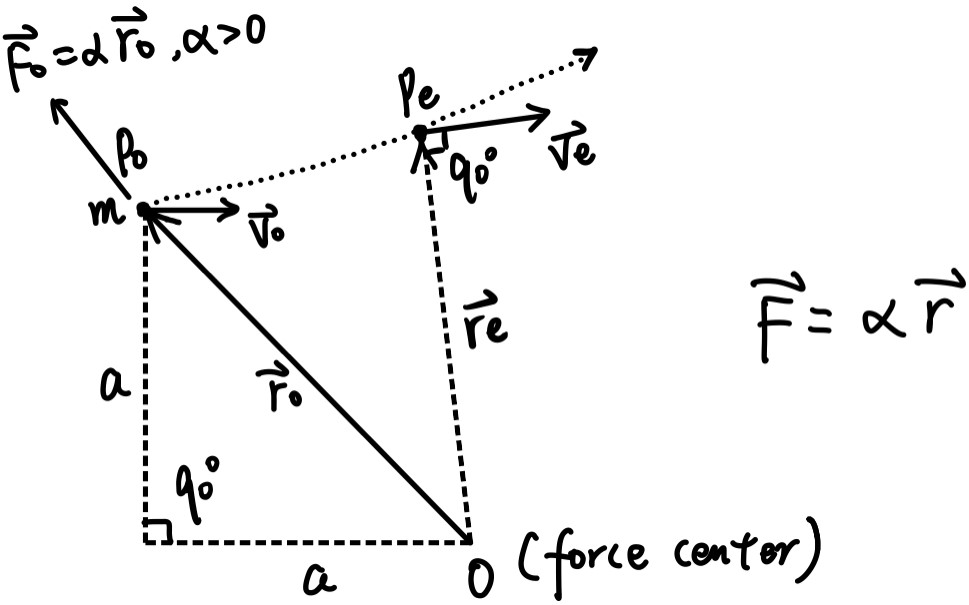
\includegraphics[width=0.4 \linewidth, angle =0]{ex1.png}
%\caption{.}
\label{fig:3}
\end{figure}
\end{frame}

\section{Rigid Body Dynamnics Part I}
\begin{frame}
  \begin{block}{Rigid Body}
    A body is called rigid if $|\vec{r_i}-\vec{r_j}| = \text{const}$ for any point $i, j$ in the body.
  \end{block}\pause
  Degree of freedom of a rigid body?\pause
  \begin{figure}[htbp]
  \centering
  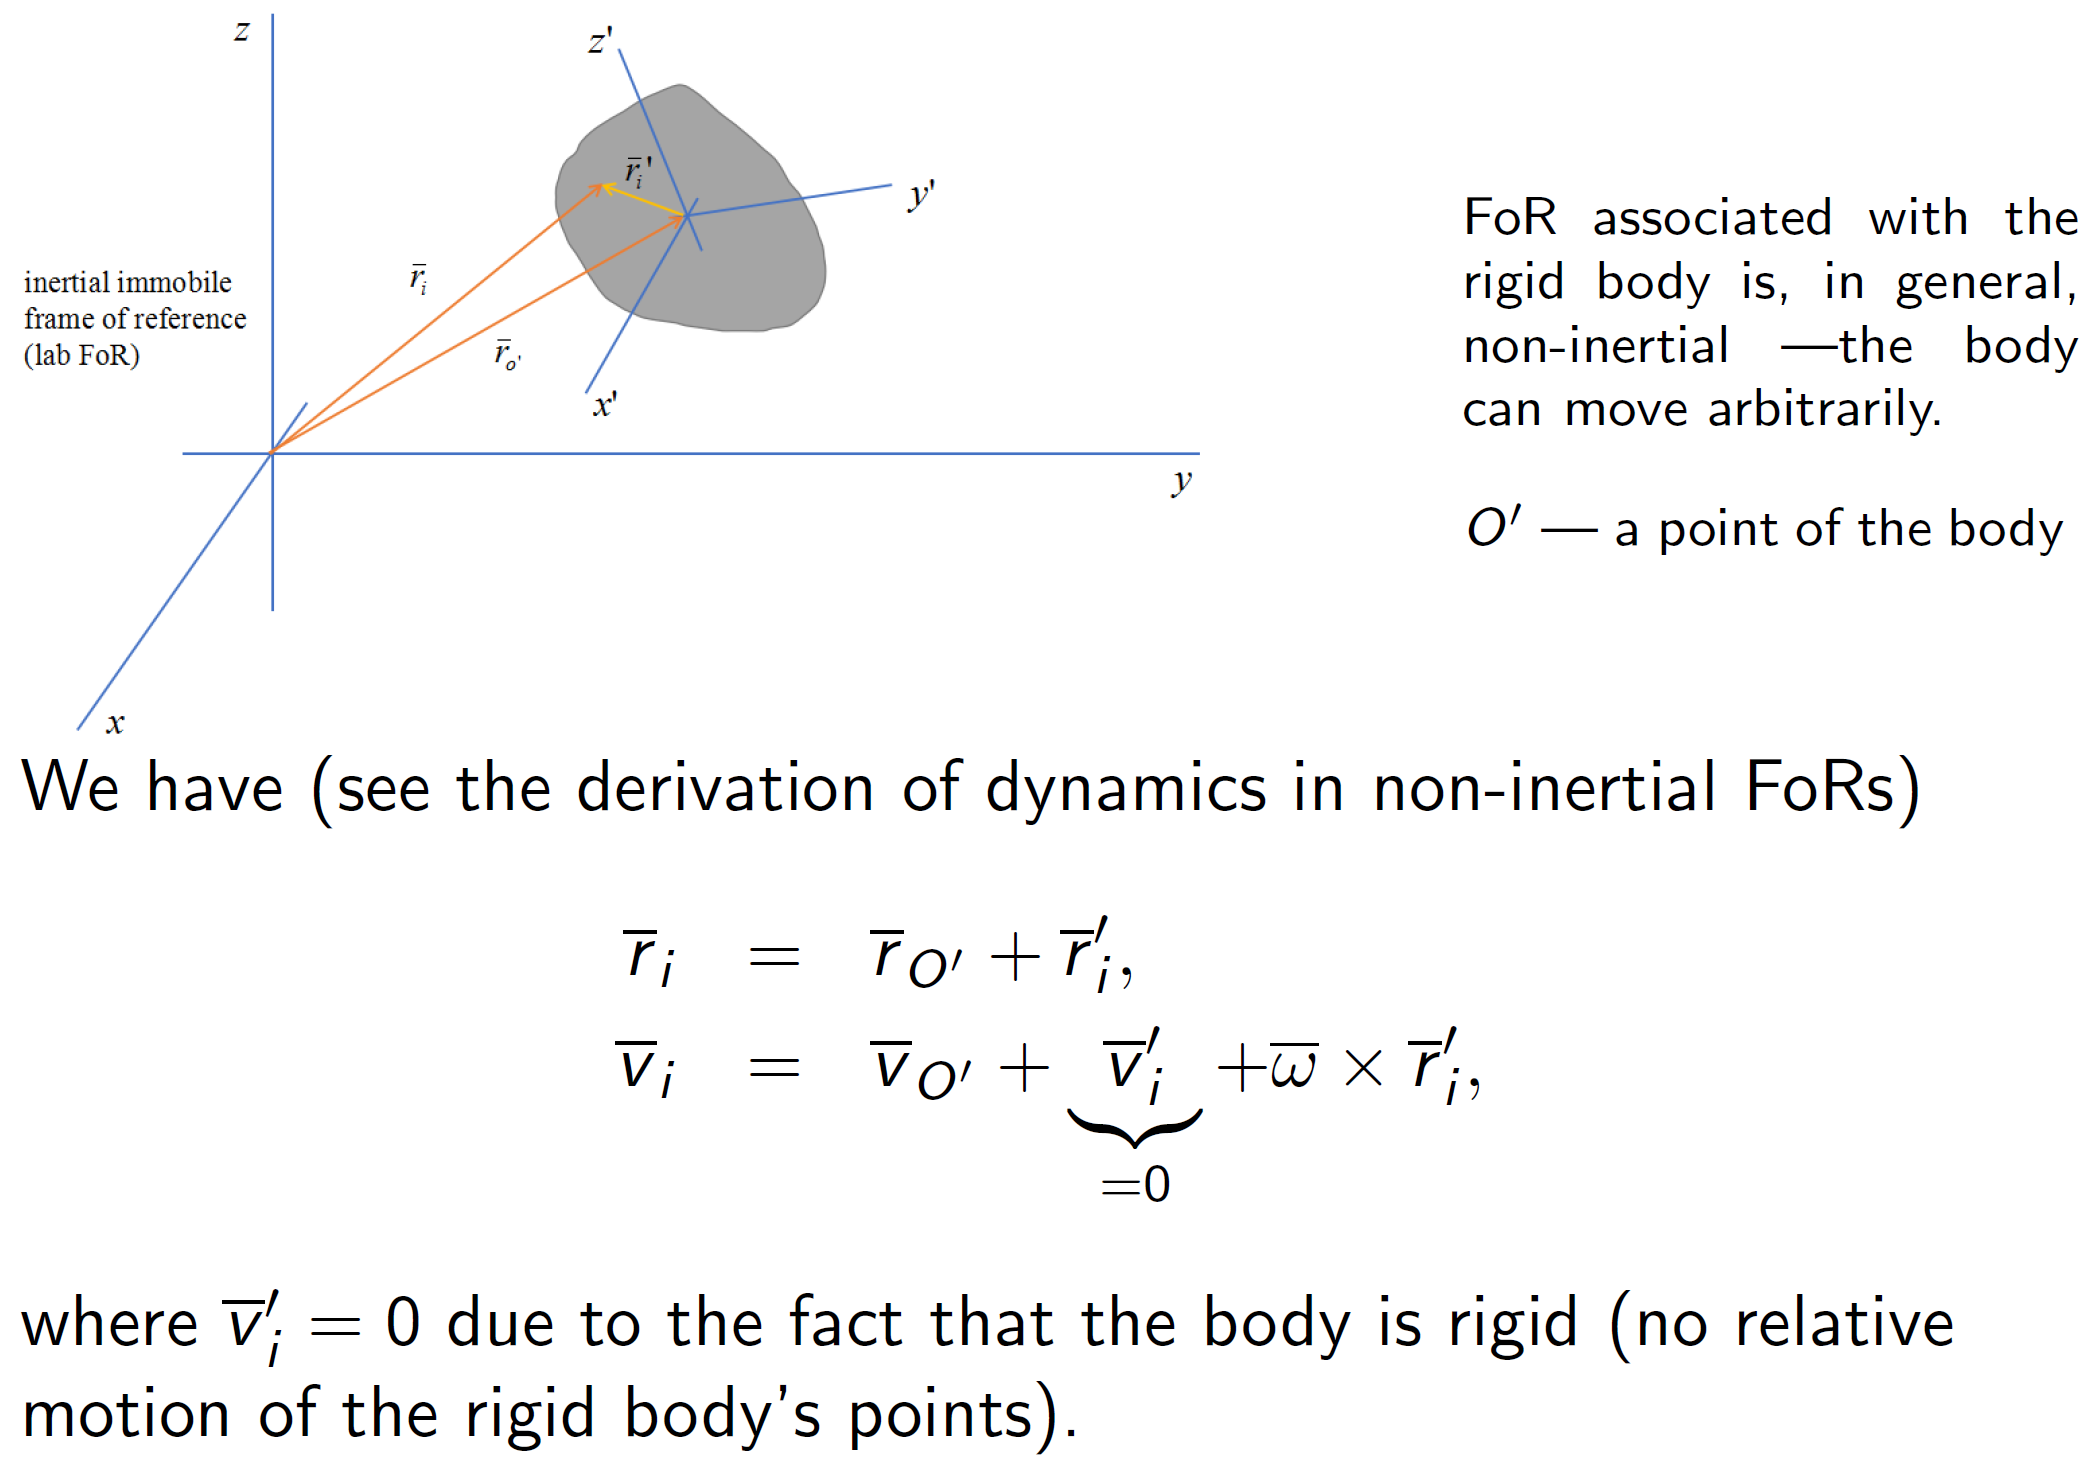
\includegraphics[width=0.7 \linewidth, angle =0]{rigid.png}
  %\caption{.}
  \label{fig:4}
  \end{figure} 
\end{frame}

\begin{frame}
  \begin{figure}[htbp]
  \centering
  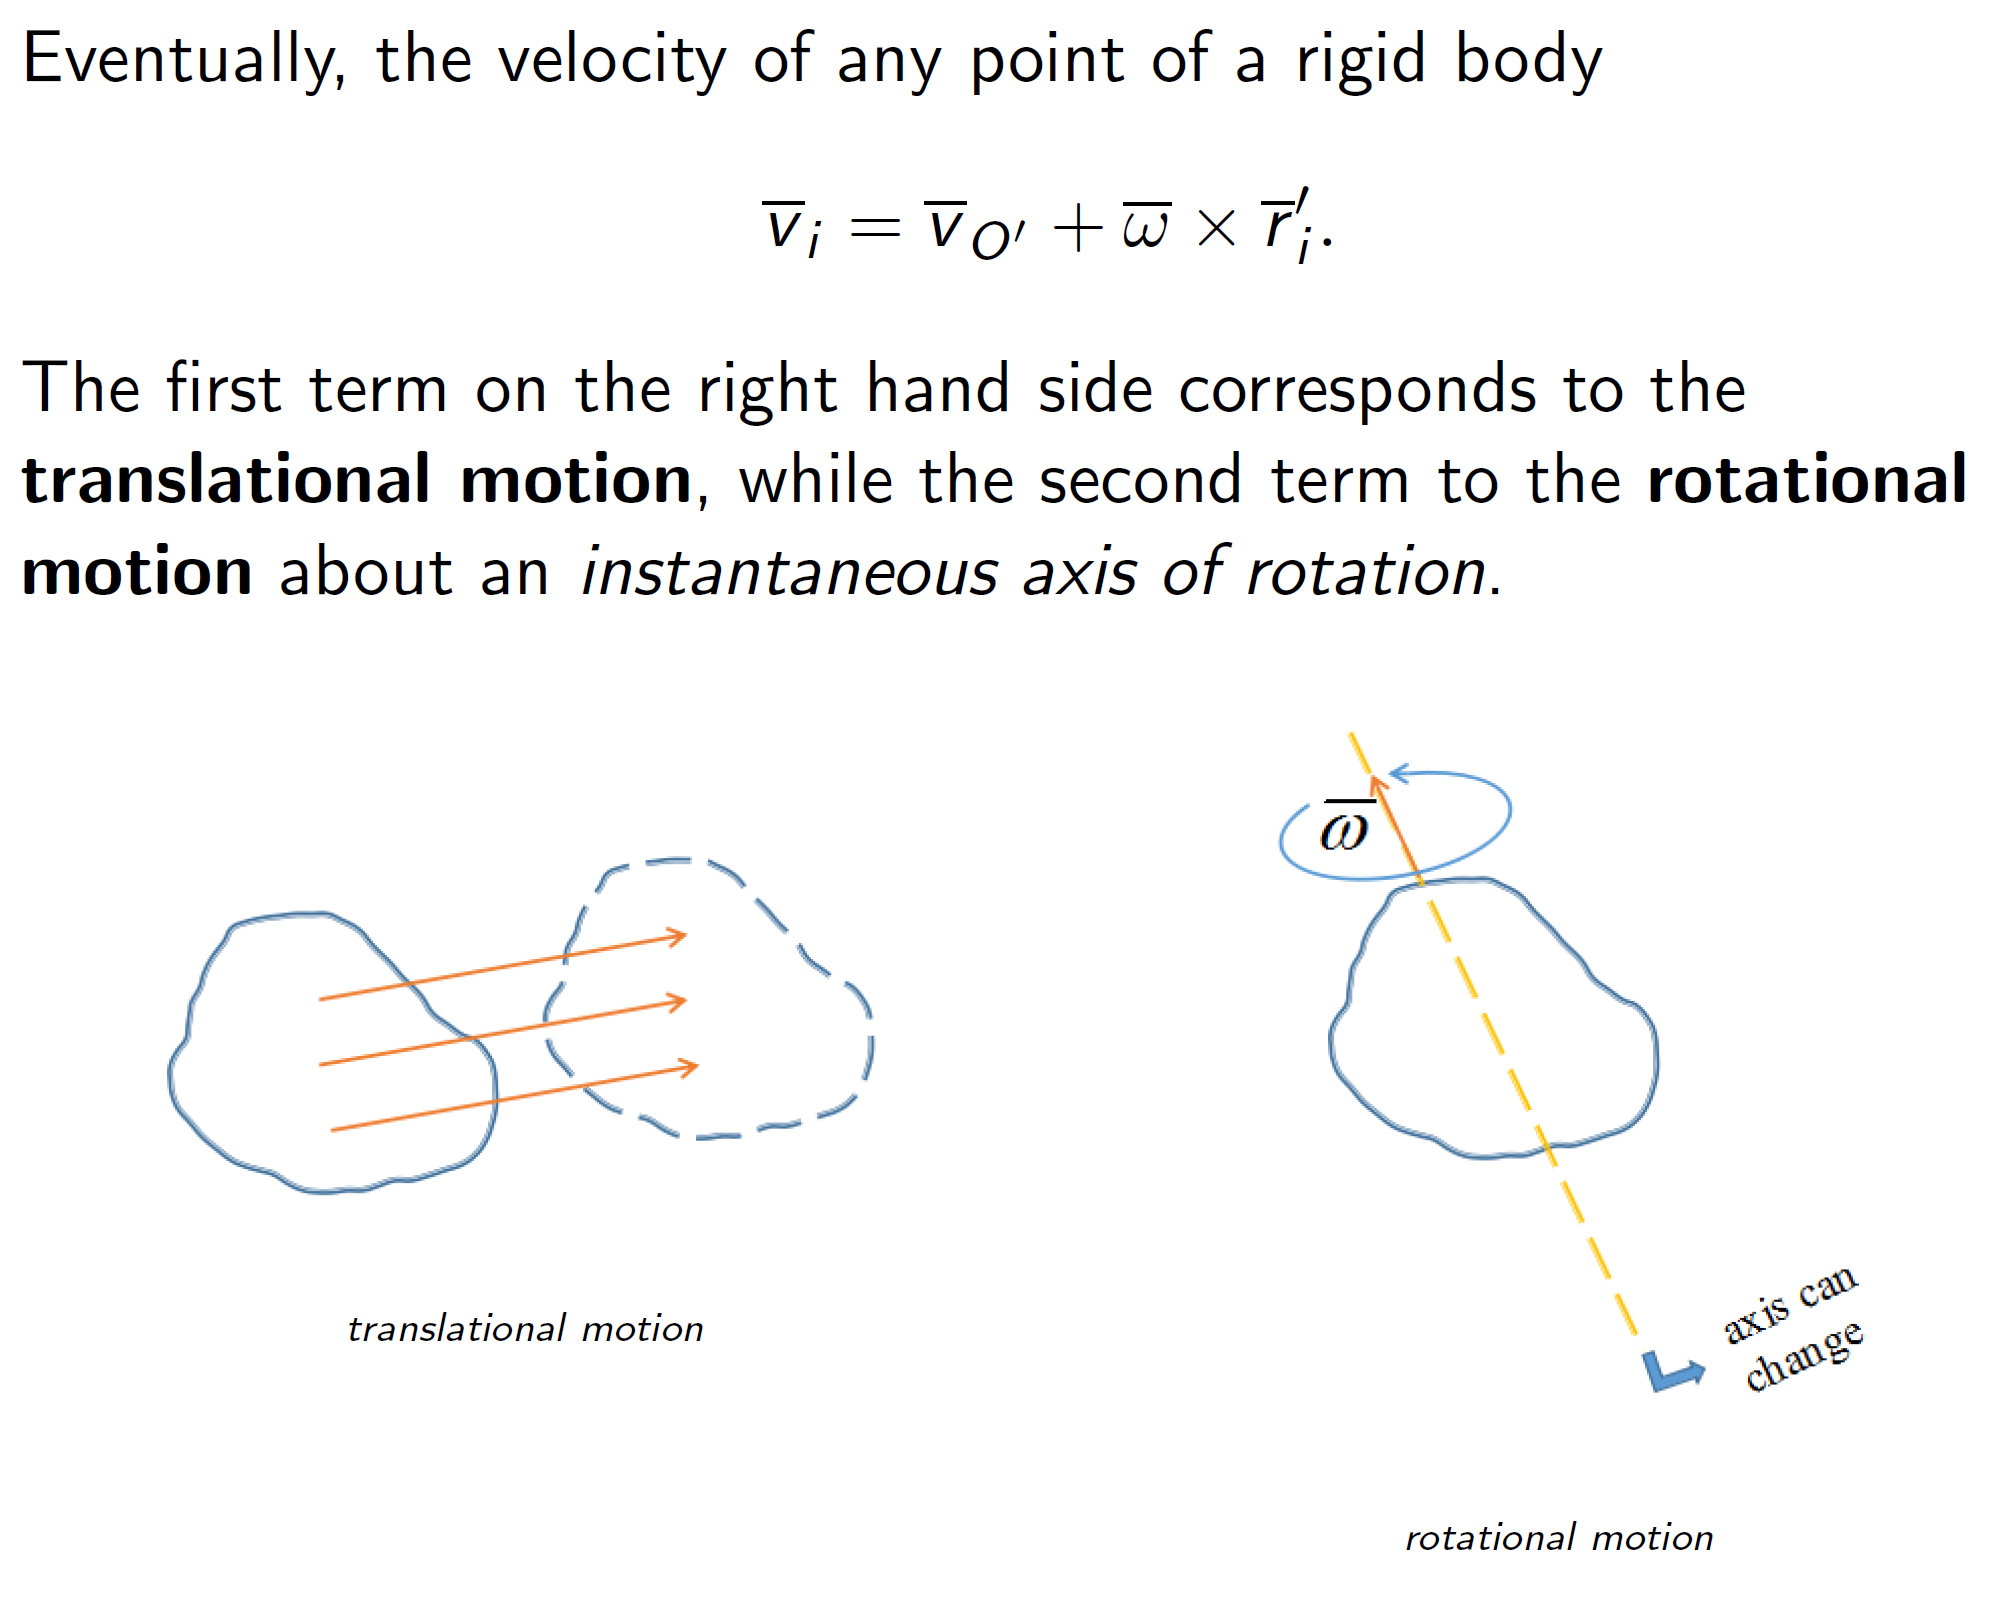
\includegraphics[width=0.8 \linewidth, angle =0]{rigid2.png}
  %\caption{.}
  \label{fig:5}
  \end{figure}
\end{frame}

\begin{frame}
  \begin{figure}[htbp]
  \centering
  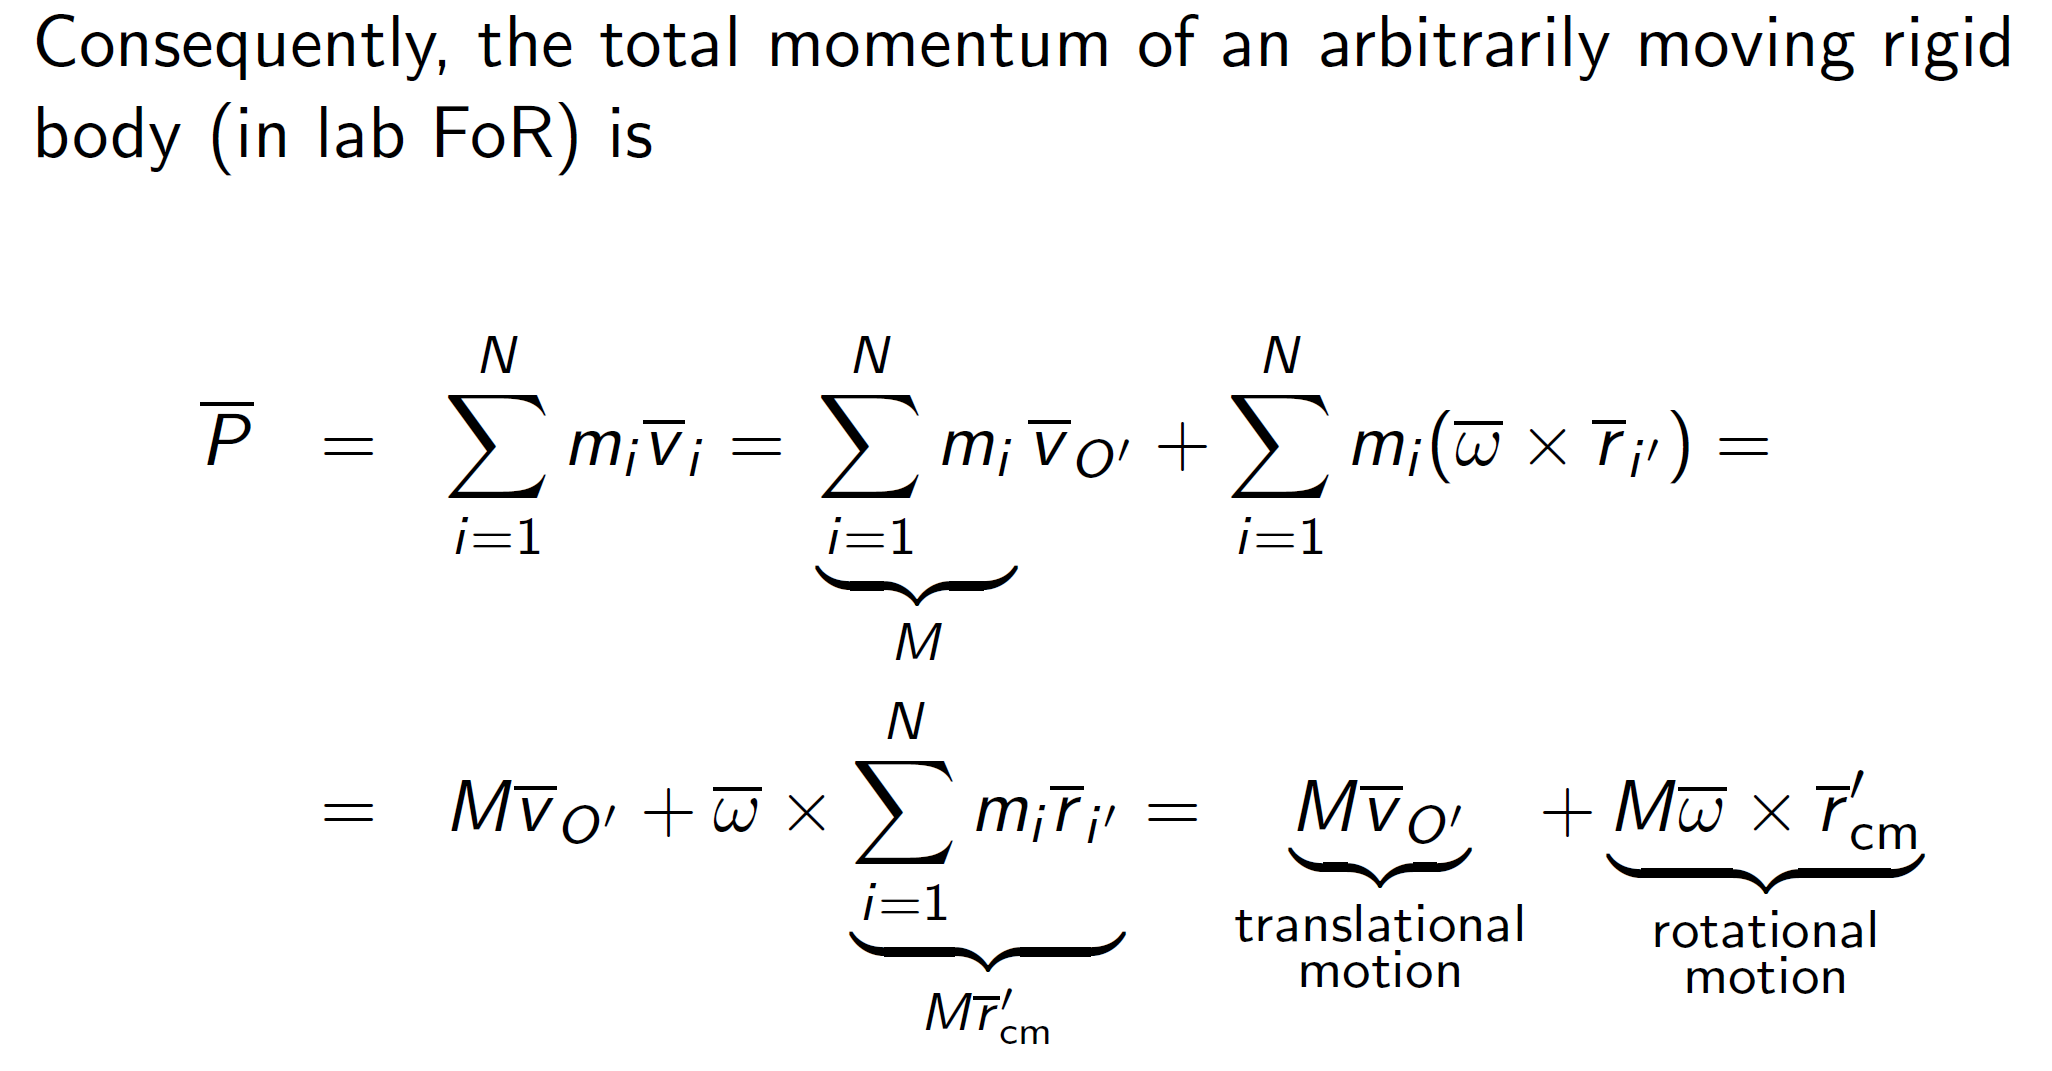
\includegraphics[width=0.8 \linewidth, angle =0]{rigid3.png}
  %\caption{.}
  \label{fig:6}
  \end{figure}\pause
  \textcolor{blue}{$$\Rightarrow \vec{p} = M\vec{v_c}$$}
\end{frame}

\begin{frame}
  \begin{figure}[htbp]
  \centering
  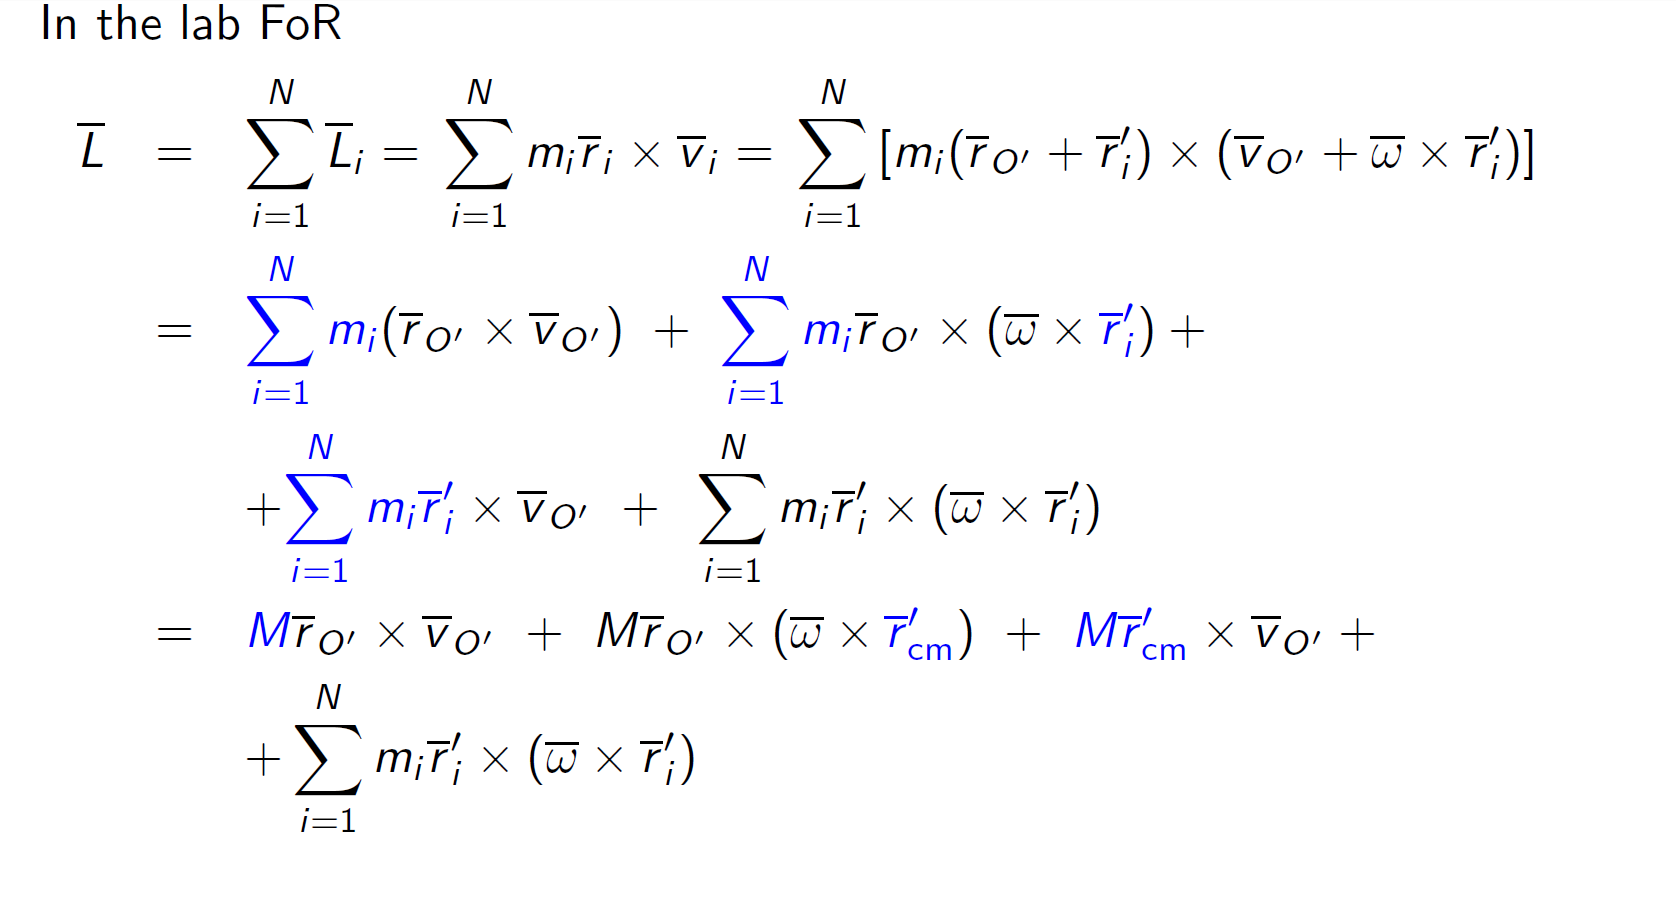
\includegraphics[width=0.7 \linewidth, angle =0]{rigid4.png}
  %\caption{.}
  \label{fig:7}
  \end{figure}\pause
 $$\Rightarrow \vec{L} = \underbrace{\vec{L_c}}_{=M\vec{r_c}\times \vec{v_c}} + \vec{L'}$$\pause
 $\vec{L'} = \sum_{i=1}^{N} m_{i} \bar{r}_{i}^{\prime} \times\left(\bar{\omega} \times \bar{r}_{i}^{\prime}\right)$: Rigid body's angular momentum w.r.t its center of mass 
\end{frame}

\begin{frame}{Tensor of Inertia}
  $$\vec{L'} = \sum_{i=1}^{N} m_{i} \bar{r}_{i}^{\prime} \times\left(\bar{\omega} \times \bar{r}_{i}^{\prime}\right) = I\vec{\omega}$$\pause
  $$\begin{gathered}
    {I=\left[\begin{array}{lll}
    I_{x^{\prime} x^{\prime}} & I_{x^{\prime} y^{\prime}} & I_{x^{\prime} z^{\prime}} \\
    l_{y^{\prime} x^{\prime}} & I_{y^{\prime} y^{\prime}} & I_{y^{\prime} z^{\prime}} \\
    I_{z^{\prime} x^{\prime}} & I_{z^{\prime} y^{\prime}} & I_{z^{\prime} z^{\prime}}
    \end{array}\right]=} \\
    {\left[\begin{array}{lll}
    \sum_{i=1}^{N} m_{i}\left(y_{i}^{\prime 2}+z_{i}^{\prime 2}\right) & \sum_{i=1}^{N} -m_{i} x_{i}^{\prime} y_{i}^{\prime} & \sum_{i=1}^{N} -m_{i} x_{i}^{\prime} z_{i}^{\prime} \\
    \sum_{i=1}^{N} -m_{i} y_{i}^{\prime} x_{i}^{\prime} & \sum_{i=1}^{N} m_{i}\left(x_{i}^{\prime 2}+z_{i}^{\prime 2}\right) & \sum_{i=1}^{N} -m_{i} y_{i}^{\prime} z_{i}^{\prime} \\
    \sum_{i=1}^{N} -m_{i} z_{i}^{\prime} x_{i}^{\prime} & \sum_{i=1}^{N} -m_{i} z_{i}^{\prime} y_{i}^{\prime} & \sum_{i=1}^{N} m_{i}\left(x_{i}^{\prime 2}+y_{i}^{\prime 2}\right)
    \end{array}\right]}
    \end{gathered}$$\pause
    \textcolor{blue}{$\vec{L}$ can not be always parallel to $\vec{\omega}$, when will it be?\\
    By a random choice of $x', y', z'$, e.g. \textbf{$\omega_x', \omega_y',\omega_z'$ all contributes to $\vec{\mathbf{L_x'}}$}, it's hard to see, but if we ...}
  \end{frame}

\begin{frame}
  By choosing a better set of $\tilde{x}^{\prime}, \tilde{y}^{\prime}, \tilde{z}^{\prime}$, we can obtain a diagonal form of $I$.
  $$I=\left[\begin{array}{ccc}
    I_{\tilde{x}^{\prime} \tilde{x}^{\prime}} & 0 & 0 \\
    0 & I_{\tilde{y}^{\prime} \tilde{y}^{\prime}} & 0 \\
    0 & 0 & l_{\tilde{z}^{\prime} \tilde{z}^{\prime}}
    \end{array}\right]$$\pause
    \textcolor{blue}{Then, \textbf{$\omega_x'$ only contributes to $\vec{\mathbf{L_x'}}$, so do $\omega_y'$ and $\omega_z'$}}
    $$\Rightarrow L_{x^{\prime}}=I_{\tilde{x}^{\prime} \tilde{x}^{\prime}}\cdot \omega_{x^{\prime}}, \quad L_{y^{\prime}}=I_{\tilde{y}^{\prime} \tilde{y}^{\prime}} \cdot \omega_{y^{\prime}}, \quad L_{z^{\prime}}=I_{\tilde{z}^{\prime} \tilde{z}^{\prime}} \cdot \omega_{z^{\prime}}$$\pause
    The axis in this special sets of axes is called the \textbf{Pricipal axis}, which is our main focus.
\end{frame}

\begin{frame}{How to find principle axis}
  \begin{enumerate}
    \item Find the mass center $C$ of the rigid body, let $C$ be the origin\pause
    \item Use the current coordinates $x, y, z$ to derive the tensor of inertia $I$\pause
    \item Let $det(I-\lambda \mathbb{1}) = 0$ to find $\lambda_1, \lambda_2, \lambda_3$.\pause
    \item Plug back $\lambda_i$ into the equation $(I - \lambda_i\mathbb{1})\vec{u_i} = 0$, find the solution $\vec{u_1},\vec{u_2},\vec{u_3}$\pause
    \item Use the direction of $\vec{u_1},\vec{u_2},\vec{u_3}$ as axes, calculate the new $I_p$.
  \end{enumerate}

  
  \begin{itemize}
    \item \textcolor{blue}{Use symmetry to "guess" the principle axes.}\pause
    \item \textcolor{blue}{Why does this methods always works?}\pause
    \item \textcolor{blue}{Recall the form of $I$, it's a self-adjoint matrix.\\
    To learn the mathematical details, have a look at:}\\ 
    zxj\_Eigenvalue \& Diagonalization.pdf (under canvas RC folder).
    %\href{umjicanvas.com/courses/2075/files/folder/RC/Ren%20Zeyi?preview=544006}
  \end{itemize}
\end{frame}

\begin{frame}
\textcolor{blue}{Exercise 2}

Use the example in slide(s-21hp14) to practice.
\begin{figure}[htbp]
\centering
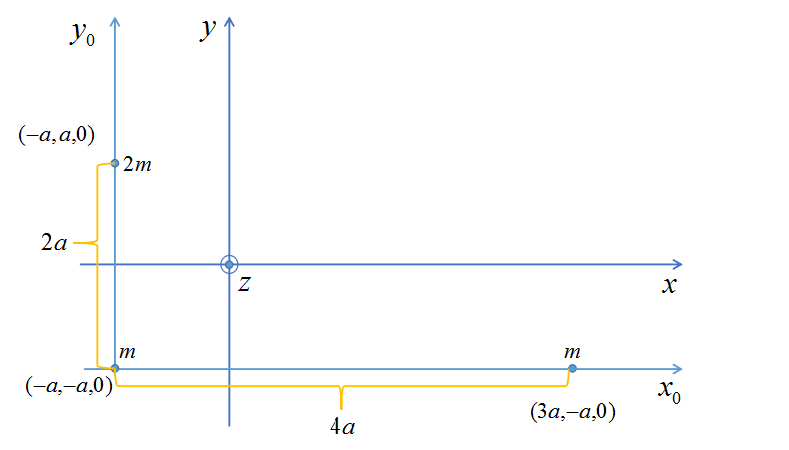
\includegraphics[width=0.5 \linewidth, angle =0]{ex2.png}
%\caption{.}
\label{fig:8}
\end{figure}
(answer: in slide)
\end{frame}

\begin{frame}{Reference}
  \begin{thebibliography}{9}
  \setbeamertemplate{bibliography item}[article]
  \bibitem{C} Yigao Fang.\\
  \textcolor{black}{VP160 Recitation Slides.}\\
  2020
  \bibitem{C} Haoyang Zhang.\\
  \textcolor{black}{VP160 Recitation Slides.}\\
  2020
  % \setbeamertemplate{bibliography item}[book]
  % \bibitem{C} Yousheng Shu (舒幼生).\\
  % \textcolor{black}{\textit{Mechanics (力学)}}\\
  % Peking University Press, 2005
  % \setbeamertemplate{bibliography item}[book]
  % \bibitem{C} Jiafu Cheng (程稼夫).\\
  % \textcolor{black}{\textit{中学奥林匹克竞赛物理教程:力学篇}}\\
  % University of Science and Technology Press, 2013
  \end{thebibliography}
  \end{frame}
  \end{document}



